The proposed controller design for this work has 3 major goals derived from
requirements and challenges faced with a neural implementation in
\cite{HuntPhDThesis}. See \myref{chap:introduction} for more details.

\begin{enumerate}
\item Decrease torque errors between neuron desired model and executed torques
\item Minimize phase shift between desired and achieved trajectory
\item Decrease position error during trajectory execution to less than 5 degrees from the desired position
\end{enumerate}

Requirement 1 is fulfilled in
the controller through sensor fusion to estimate state at the time of sensor
readings (assumed to be ``current" time) and then using an internal model of the
joint's dynamics to predict the evolution of the joint's position and velocity
given a particular controlling torque. From there, an internal optimization loop
can run to identify a goal torque with sufficient resolution.

An accurate internal model will help meet all 3 requirements. In particular, an
internal model directly solves Requirement 1 by matching controlled torques to
pressures accounting for the pneumatic muscle dynamics. The internal model
designed into the control is designed to adapt to the actual observed
characteristics of the joint, allowing for changing dynamics over time (for
example, adding or removing weight from the robot, degrading pneumatic muscles
or changing positions of other limbs),
adapting to different joints with the same controller and increasing the
robustness of the controller to variations from the original estimated
properties of the robot. The accurate internal model also avoids a phase shift for Requirement 2. 

Requirement 3 is met by a combination of the design decisions above and
constitutes a metric by which to measure the effectiveness of the new design
relative to previous designs, regardless of implementation.

\bbs{Sensor Fusion}

Within the controller, state estimation is done in a relatively simplified
manner. The design trades off increased accuracy for reduced computation time. The 
estimation is designed to have sufficiently small error that it would not adversely impact rest of the system. An additional consideration
was the ability to implement the algorithm in a neuron system.

\subsection{Central Divided Difference}

The velocity was estimated with a fixed window of the last 3 position readings.
From there, a central divided difference formula was used to estimate the
slope and estimate velocity. This was found to be more accurate than a forward
divided difference method only incorporating two points in practice when run
against simulated data.

The equation that defines the centered divided difference:

\begin{equation}
\dot{\theta} = \dfrac{\theta_{t} - \theta_{t - 2}}{2 \delta t}
\end{equation}

\subsection{Pneumatic Actuator Modeling}

The internal estimation of the current acceleration was primarily based on the 
pressure sensors on the robot. These readings, combined with a position sensor, 
allow for direct measurements of the state of the actuator and therefore the
applied torque. The model comes from \cite{HuntPMuscles}.

To calculate a pressure from a force and position, the following model is used:

\begin{equation}
P = a_{0} + a_{1} * tan(a_{2} (\dfrac{k}{a_{4} * F + k_{max}} + a_{3})) + a_{5} * F + a_{6} * S
\end{equation}

The terms used within the overall model are defined as follows:

\begin{equation}
k_{max} = \dfrac{L_{rest} - L_{620 kPa}}{L_{rest}}
\end{equation}

The $k_{max}$ term defines the maximum strain. This occurs at the maximum pressure for the actuator, 620 kPa. The $k$ term defines the strain at the current position.

\begin{equation}
k = \dfrac{L_{rest} - L_{angle}}{L_{rest}}
\end{equation}

The length for the current angle $L_{angle}$ is calculated as follows:

\begin{equation}
L_{angle} = L_{0} - L_{1} cos(\alpha + \theta)
\end{equation}

The force required by the actuator is calculated from the joint torque at the current joint state.

\begin{equation}
F = \dfrac{T}{d cos(\beta + \theta)}
\end{equation}

$\alpha, \beta, d, L_{rest}$ and $L_{620 kPa}$ represent the parameters for a 
particular actuator. The $a$ values represent optimized parameters
for the generalized model that adjusts to all actuators. These values for $a_{1}$ to $a_{6}$ are taken directly from \cite{HuntPMuscles}.

There are 3 key aspects to the model. First, the over model is a shifted and 
scaled tangent curve. This represents the observed trend that increasing 
pressure has less strain effects for short changes in length or large changes in 
length, with an stronger effect for medium changes in length. This is similar to 
the behavior of biological muscles.

Second, The scaling effect comes from the observed
effect that increased end effector force leads to a shrinking of the tangent 
curve.

Third, there is a hysteresis term ($a_{6} * S$) that represents the internal
friction observed in the filling and emptying process.

From there, the estimation of acceleration comes from the mass, 
damping and conservative forces and the torque model specified in
\myref{chap:lit_review}.

\bbs{Optimizing Torque Control}

Once the current state of the robot was determined, the optimization process was 
done recursively using a binary search algorithm. 

This equation and model are designed to present a forward model to convert from 
a desired torque and force to a pressure. There is not a clean and simple 
inversion of the model; however, a binary search algorithm 
(\myref{fig:BinarySearch}, \github{stability/torque\_projection.py}) was used to invert 
the process by estimating a maximum and minimum torque to apply and narrowing 
the
potential window from there. This allows for a estimating a known bound on the 
potential error and balancing the error with how quickly the algorithm iterates.

\begin{figure}
\centering
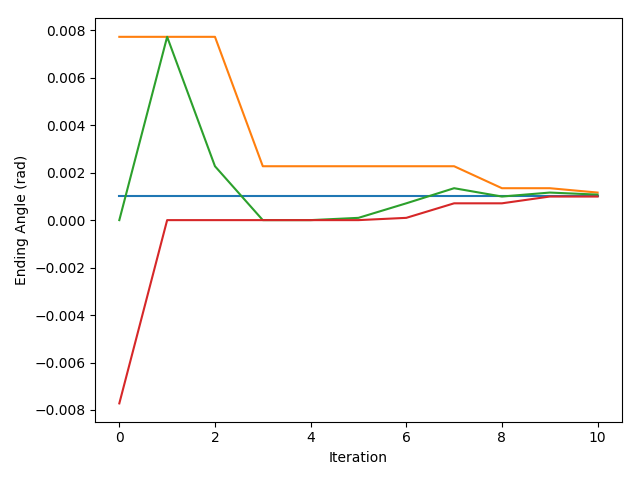
\includegraphics[width=5in]{controller_design/BinarySearch}
\caption{Optimize torque control with binary search. The orange and red lines are upper and lower bounds respectively, with the current estimate shown in green}
\label{fig:BinarySearch}
\end{figure}

Bounds were selected from estimates
of the maximum and minimum (maximum negative) torque that can be applied to the
joint. From there, a forward projection mechanism based on the internal physics model was
used to estimate the resulting position. From there, the binary search procedure
repeatedly shrinks the bounds around the optimal torque. The model can be 
applied to each actuator in the pair independently (with a fixed antagonistic 
torque) or as a pair with a variable overlap in torque. 

The final
step is to convert the desired torque into a pressure control. This conversion takes
one final forward iteration of the model above, at the current joint angle, to 
calculate the desired pressure for each of the actuator.

\subsection{Forward Projection of State}

Given the current state and an applied torque, the joint model in 
\myref{chap:lit_review} can be used to predict the motion of the joint.
This was done at multiple time resolutions, with increased time resolution 
increasing the accuracy of the internal prediction. This is a direct trade-off;
however, a more accurate internal prediction directly increases the tracking
performance of the algorithm.

One aspect of the current algorithm that allows for reduced fidelity is the 
opportunity to make estimates for an upper and lower bound. This allows the 
controller to bound the maximum possible positional error and iterate further
if there is insufficient accuracy at particular steps.

\subsection{Torque to Pressure}

Converting from a desired torque to pressure for a single actuator follows
the model expressed above:

\begin{equation}
P = a_{0} + a_{1} * tan(a_{2} (\dfrac{k}{a_{4} * F + k_{max}} + a_{3})) + a_{5} * F + a_{6} * S
\end{equation}

One complicated aspect of implementing conversion from the desired torque to 
pressures for
the joint is incorporating the antagonistic overlap of the actuation of the two 
muscles. It is often sufficient to pick a fixed overlap for the joints; however,
there is room for improvement for varying the overlap and stiffness of the joint.

Another complicated aspect of designing desired pressure in the system is the
knowledge of the underlying control scheme. As mentioned in \cite{HuntPMuscles},
the underlying controller implements a bang-bang algorithm. This means that 
there is some uncontrolled variation; however, a more complicated algorithm
can use the understanding that there is a fixed controlled window.

\bbs{System Modeling}

One of the key aspects of the control design is the internal estimate of key 
joint parameters. These have been simplified down to 3 key parameters: inertia 
($M$), damping ($C$) and conservative load ($N$). The simplified internal 
model uses the following equation to determine the acceleration of the joint:

\begin{equation}
M * \ddot{\theta} + C * \dot{\theta} + N * sin(\theta) = \tau
\end{equation}

\begin{equation}
\ddot{\theta} = \dfrac{\tau - C * \dot{\theta} - N * sin(\theta)}{M}
\end{equation}

From there, the velocity and position are estimated as follows:

\begin{equation}
\dot{\theta}_{1} = \dot{\theta}_{0} + \ddot{\theta} \delta t
\end{equation}

\begin{equation}
\dot{\theta}_{avg} = \dfrac{\dot{\theta}_{0} + \dot{\theta}_{1}}{2}
\end{equation}

\begin{equation}
\theta_{1} = \theta_{0} + \dot{\theta}_{avg} \delta t
\end{equation}

Using this model, the estimated acceleration between now and the next controller 
step is predicted and compared with the observed acceleration. On the other hand,
there is not a sensor that directly observes joint acceleration. Instead, error
is measured in the difference in the estimated position and the measured 
position.

\bbss{Acceleration Error}

\begin{equation}
\ddot{\theta}_{act} = \dfrac{\tau}{M} - \dfrac{C \dot{\theta}_{0}}{M} - \dfrac{N sin(\theta)}{M}
\end{equation}

\begin{equation}
(\ddot{\theta}_{act} + \ddot{\theta}_{err}) = \dfrac{(\tau + \tau_{err})}{(M + M_{err})} - \dfrac{(C + C_{err}) (\dot{\theta}_{0} + \dot{\theta}_{err})}{(M + M_{err})} - \dfrac{((N + N_{err})sin(\theta + \theta_{err}))}{(M + M_{err})}
\end{equation}

This equation includes some sources of error that are assumed to be small. In 
this analysis, the mass error $M_{err}$ is assumed to be small because it can
be measured directly from the robot. $\tau_{err}$ is assumed to be small because
the underlying pressure controller is assumed to correctly apply pressures to
match the calculated desired torque. In general, the assumption is that the error
comes primarily from errors in the damping and conservative load estimate. This 
assumption may not be correct, but continued effort on estimation (in particular 
velocity estimation) will hope to minimize estimation errors (potentially by 
including concepts from Kalman filtering).

The revised, simplified equation that assumes error comes from parameter estimation is as follows:

\begin{equation}
(\ddot{\theta}_{act} + \ddot{\theta}_{err}) = \dfrac{\tau}{M} - \dfrac{(C + C_{err})}{M}\dot{\theta}_{0} - \dfrac{(N + N_{err})sin(\theta)}{M}
\end{equation}

The error components can be identified by subtracting out the non-error 
components:

\begin{equation}
(\ddot{\theta}_{act} + \ddot{\theta}_{err}) - \ddot{\theta}_{act} =
\dfrac{\tau}{M} - \dfrac{\tau}{M}
- \dfrac{(C + C_{err})}{M}\dot{\theta}_{0} + \dfrac{C}{M}\dot{\theta}_{0}
- \dfrac{(N + N_{err})sin(\theta)}{M}  + \dfrac{N sin(\theta)}{M}
\end{equation}

The terms above are gathered to highlight $C_{err}$ and $N_{err}$, the terms representing the error in the internal estimation of damping and static load.

\begin{equation}
\ddot{\theta}_{err} =
- C_{err} \dfrac{\dot{\theta}_{0}}{M}
- N_{err} \dfrac{sin(\theta)}{M}
\end{equation}

\begin{equation}
\ddot{\theta}_{err} = - \dfrac{1}{M}
(C_{err} \dot{\theta}_{0} + N_{err} sin(\theta))
\end{equation}

\bbss{Velocity Error}

Following the assumptions above, errors in internal estimation can be propagated to be measured from errors in velocity.

\begin{equation}
(\dot{\theta}_{1, act} + \dot{\theta}_{1, err}) = \dot{\theta}_{0} + (\ddot{\theta}_{act} + \ddot{\theta}_{err}) \delta t
\end{equation}

\begin{equation}
\dot{\theta}_{1, err} = \ddot{\theta}_{err} \delta t
\end{equation}

\begin{equation}
\dot{\theta}_{1, err} = - \dfrac{\delta t}{M}(C_{err} \dot{\theta}_{0} + N_{err} sin(\theta))
\end{equation}

\begin{equation}
(\dot{\theta}_{avg, act} + \dot{\theta}_{avg, err}) = \dfrac{\dot{\theta}_{0} + (\dot{\theta}_{1, act} + \dot{\theta}_{1, err})}{2}
\end{equation}

\begin{equation}
\dot{\theta}_{avg, err} = \dfrac{\dot{\theta}_{1, err}}{2}
\end{equation}

\begin{equation}
\dot{\theta}_{avg, err} = - \dfrac{\delta t}{2M}(C_{err} \dot{\theta}_{0} + N_{err} sin(\theta)) = \dfrac{\delta t}{2} \ddot{\theta}_{err}
\end{equation}

\bbss{Positional Error}

Following the assumptions above, errors in internal estimation can be propagated to be measured from errors in position. This assumes that the primary source of error comes from the acceleration and velocity and that the estimate of the current position is comparatively accurate.

\begin{equation}
(\theta_{1, act} + \theta_{err}) = \theta_{0} + (\dot{\theta}_{avg} + \dot{\theta}_{avg, err}) \delta t
\end{equation}

\begin{equation}
\theta_{err} = \dot{\theta}_{avg, err} \delta t = \dfrac{\delta t^{2}}{2} \ddot{\theta_{err}} = - \dfrac{\delta t^{2}}{2M}(C_{err} \dot{\theta}_{0} + N_{err} sin(\theta))
\end{equation}

\begin{equation}
- \dfrac{2M}{\delta t^{2}} \theta_{err} = C_{err} \dot{\theta}_{0} + N_{err} sin(\theta)
\end{equation}

\begin{equation}
N_{err} sin(\theta) = 
- \dot{\theta}_{0} C_{err}
- \dfrac{2M}{\delta t^{2}} \theta_{err}
\end{equation}

When $\dot{\theta}_{0}$ is 0, then $N_{err} sin(\theta)$ explains the total error in acceleration. When $\dot{\theta}_{0}$ is large, $N_{err} sin(\theta)$ should explain a diminishing amount of the error. This can be thought of as finding the intersection between the given linear function and the vector $[\dot{\theta}_{0}, 1]$ scaled by a factor $\lambda$, where $C_{err}$ is the first term and 
$N_{err} sin(\theta)$ is the second term.

\begin{equation}
C_{err} = \lambda \dot{\theta}, N_{err} = \dfrac{\lambda}{sin(\theta)}
\end{equation}

\begin{equation}
\lambda = 
- \lambda \dot{\theta}_{0}^{2}
- \dfrac{2M}{\delta t^{2}} \theta_{err}
\end{equation}

\begin{equation}
\lambda (1
+ \dot{\theta}_{0}^{2})
=
- \dfrac{2M}{\delta t^{2}} \theta_{err}
\end{equation}

\begin{equation}
\lambda 
=
- \dfrac{2M}{\delta t^{2} (1 + \dot{\theta}_{0}^{2})} \theta_{err}
\end{equation}

This formulation does leave a singular point in the solution. When the joint is stopped and the joint is centered, then there are no damping or loads that apply torque to the joint. In this case, there is a check to pause updating of the internal estimate of joint parameters.

\subsection{Evaluation of asymmetric error concerns}

One additional consideration for the design of the controller is the asymmetric
effect that estimation error has on the over or under-damping behavior of the
controller. Intuitively,
underestimating the inertia of the controlled link leads to a decreased control
torque, which will make a smaller adjustment to velocity than required. On the
other hand, overestimating the mass will cause an over-application of torque
that can't be corrected until the next control iteration, potentially causing
extreme motions that go uncorrected in an under-damped control scenario.

Going back to the calculation of the acceleration from torque:

\begin{equation}
M * \ddot{\theta} = \tau - C * \dot{\theta} - N * sin(\theta)
\end{equation}

Given the desire to over-damp the system instead of under-damp the system, the
above equation informs the relative penalty of positive or negative error for
each internal parameter (including mass).

For a constant $C$ and $N$, an increased mass estimate leads to increased torque
applied. If the actual inertia is lower, the actual required torque is lower 
than the controlled torque so the system will make a larger change in velocity 
than the desired trajectory requires. This behavior can lead to under-damped 
control, therefore the preference is to underestimate the inertia of the system.

\begin{figure}
\centering
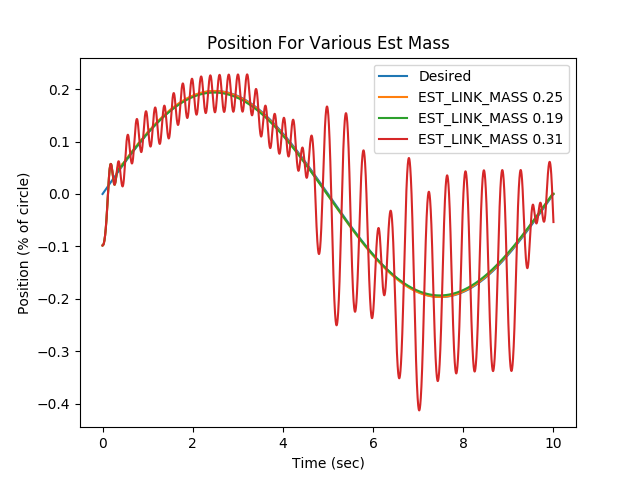
\includegraphics[width=5in]{controller_design/Tracking_Optimizing_LINK_MASS2}
\caption{Underdamped control due to mass estimate}
\label{fig:UnderdampedControl}
\end{figure}


For a constant $M$ and $N$, an increased estimate of the damping leads to 
increased torque applied. If the actual damping is lower, the actual required
torque is lower than the controlled torque, again leading to an over-correcting
system. Varying $N$ behaves the same way, except that the effects of $N$ may be
minimal when $sin(\theta)$ is small.
